\documentclass[11pt]{article}
\usepackage{geometry}

\geometry{landscape, a4paper, margin=0mm}

\usepackage{amsmath,amssymb}
\usepackage{tikz-qtree}
\usepackage{fullpage}
\usepackage{pdflscape}

\hoffset = 0pt
\voffset = 0pt
\oddsidemargin = -70pt
\topmargin = -70pt
\headheight = 0pt
\headsep = 0pt
\marginparsep = 0pt
\marginparwidth = 0pt
\footskip = 0pt
\textheight = 800pt

\newcommand{\rulefont}[1]{\ensuremath{\mathbf{(#1)}}}

\begin{document}

\pagestyle{empty}

{\footnotesize
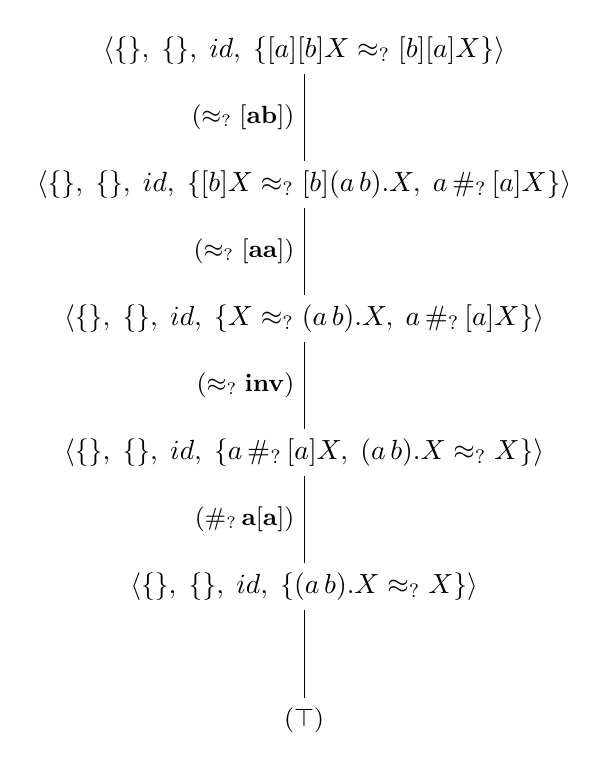
\begin{tikzpicture}[
  level distance=1.7cm,sibling distance=0.5cm,
  edge from parent path={(\tikzparentnode) -- (\tikzchildnode)}]
\tikzstyle{level 1}=[level distance=1.7cm] 
\Tree[.{$\langle\{\}, \;\{\}, \;id, \;\{[a][b]X\approx_?[b][a]X\} \rangle$}
	\edge node[auto=right] {\small $\rulefont{\approx_? [ab]}$};
[.{$\langle\{\}, \;\{\}, \;id, \;\{[b]X\approx_?[b](a\,b).X,\; a\,\#_?\,[a]X\} \rangle$}
	\edge node[auto=right] {\small $\rulefont{\approx_? [aa]}$};
[.{$\langle\{\}, \;\{\}, \;id, \;\{X\approx_?(a\,b).X,\; a\,\#_?\,[a]X\} \rangle$}
	\edge node[auto=right] {\small $\rulefont{\approx_? inv}$};
[.{$\langle\{\}, \;\{\}, \;id, \;\{a\,\#_?\,[a]X,\; (a\,b).X\approx_?X\} \rangle$}
	\edge node[auto=right] {\small $\rulefont{\#_?\, a[a]}$};
[.{$\langle\{\}, \;\{\}, \;id, \;\{(a\,b).X\approx_?X\} \rangle$} [.{\small $\rulefont{\top}$} ]]  ]
  ]
  ]
  ]
\end{tikzpicture}
}

\end{document}
